%% !TEX TS-program = xelatex
%% !TEX encoding = UTF-8 Unicode
\documentclass[12pt,a4paper]{book}
%\usepackage{fontspec} \setmainfont{Times New Roman}
%\usepackage{xeCJK} \setCJKmainfont{DFKai-SB}[AutoFakeBold]

% requires package utopia.
\usepackage{fourier}
\usepackage{amsmath,amsthm,amssymb}
\usepackage{mathtools}
\usepackage{booktabs}
\usepackage{multirow}
\usepackage[left=40mm, right=25mm, top=25mm, bottom=25mm]{geometry}
\usepackage{graphicx}
\usepackage[hidelinks]{hyperref} % colorlinks, hidelinks
\usepackage{setspace}
\usepackage{fancyhdr}
\usepackage{indentfirst}
\usepackage{titletoc}
\usepackage{titlesec}
\usepackage{appendix}
%\usepackage{lipsum}
%\usepackage{showframe}

\renewcommand{\huge}{\fontsize{22}{22}\selectfont}
\renewcommand{\LARGE}{\fontsize{18}{18}\selectfont}
\renewcommand{\Large}{\fontsize{16}{16}\selectfont}
\renewcommand{\large}{\fontsize{14}{14}\selectfont}
\renewcommand{\small}{\fontsize{10}{10}\selectfont}
\setlength{\parindent}{1.2cm}

\titlespacing{\chapter}{0pt}{-2.5em}{1.5em}
\titleformat{\section}{\Large}{\thesection}{1ex}{}
\titleformat{\subsection}{\large\it}{\thesubsection}{1ex}{}

\author{Qiqi Gu}
\newcommand{\StudentNumber}{P0907870}
\newcommand{\AcademicUnit}{School of Applied Scineces}
\newcommand{\Programme}{PhD in Computer Applied Technology}
\newcommand{\Supervisor}{Wei Ke}
\newcommand{\Cosupervisor}{}

\newcommand{\Date}{January 25, 2022} %December 31, 2021 
\title{AI-assisted Analysis Tools for Software Development}

\makeatletter

\renewcommand{\contentsname} {Table of Contents}
\setcounter{tocdepth}{4}
\setcounter{secnumdepth}{4}
\bibliographystyle{ieeetr} %acm, ieeetr, apalike

\begin{document}

\frontmatter
\titlecontents{chapter}[0pt]{\addvspace{1.0pc}}{\bf\chaptername~\thecontentslabel.\quad}{\bf}{\hfill\contentspage}
\titleformat{\chapter}[display]{\doublespacing\filcenter\LARGE\scshape}{\chaptername~\thechapter.}{0ex}{\bf\MakeUppercase}

\begin{titlepage}
	\pagestyle{empty}
	\doublespacing\begin{center}
	
\includegraphics[width=0.25\linewidth]{MPI.pdf}

	\vspace*{0.5in}

	{\huge Macao Polytechnic Institute}

	\vspace*{0.75in}

	{\LARGE \AcademicUnit}

	\vspace*{0.75in}

	{\Large \@title}

	\vspace*{0.75in}

	\large
	\@author\\
	\StudentNumber

	\vspace*{0.75in}
		
	%{\it Thesis submitted to \AcademicUnit\ in Partial Fulfillment of the Requirements for the \Programme}
	{\it A research proposal submitted for the Confirmation of Candidature in partial fulfillment of the requirements for the degree of\\\Programme}
		
	\vfill

	\the\year
\end{center} \cleardoublepage
	\doublespacing\begin{center}
	
\includegraphics[width=0.25\linewidth]{MPI.pdf}
		
	\vspace*{2in}

	\@title
	
	\vfill

	\begin{tabular}{ll}
		Name of Student: & \@author\\
		\midrule
		Student Number: & \StudentNumber\\
		\midrule
		Academic Unit: & \AcademicUnit\\
		\midrule
		Programme: & \Programme\\
		\midrule
		Supervisor & \Cosupervisor\\
		\midrule
		Co-Supervisor: & \Supervisor\\
		\midrule
		Date: & \Date
	\end{tabular}
\end{center} \cleardoublepage
	\doublespacing\chapter*{Declaration}
\thispagestyle{empty}

I declare that this thesis has been composed solely by myself, that the work contained herein is my own except where explicitly stated otherwise in the text, and that this work has not previously been submitted in part or in full for this degree or any other degree.

I declare that I am aware of and understand the Macao Polytechnic Institute Guidelines for Plagiarism Avoidance, Rules Regarding Cheating and Other Violations of Examination Regulations, and rules and regulations related to students' academic integrity. \cleardoublepage
\end{titlepage}

\pagestyle{fancy}
\fancyhf{}
\fancyhead[C]{\small\textsc{\nouppercase\leftmark}}
\fancyfoot[C]{\small\thepage}
\begin{titlepage}
	\let\cleardoublepage\clearpage
	\pagenumbering{roman}
	\doublespacing\chapter{Abstract}

A smart contract is a program running on a blockchain platform.
Businesses often use it as a signed contract or an agreement to regulate the stakeholders
because smart contracts reduce the need in trusted intermediators, arbitrations, and enforcement costs.
Since there are existing conventional applications running business logic,
it is ideal to transform these applications to smart contracts.

Due the properties of blockchains and smart contracts, we do not think all conventional applications can be safely transformed to smart contracts.
Thus in this paper we propose to identify the patterns of conventional applications and tell which is transformable.
Then we implement algorithms to transform these applications to smart contracts.

\textbf{\textit{Keywords ---}} neural networks, smart contract, blockchain
	%\onehalfspacing\chapter*{\fontsize{22}{22}摘要}
\fontsize{14}{14}

繁體, 简体\\

\textbf{\textit{關鍵詞:}} 詞一,詞二,詞三
	\onehalfspacing\tableofcontents \addcontentsline{toc}{chapter}{\contentsname}
	\onehalfspacing\listoffigures \addcontentsline{toc}{chapter}{\listfigurename}
	\onehalfspacing\listoftables \addcontentsline{toc}{chapter}{\listtablename}
\end{titlepage}

\mainmatter

	\pagenumbering{arabic}
	\doublespacing\chapter{Introduction}

%Software development is the process of creating, specifying, programming, testing, and supporting software involved in creating and maintaining applications, frameworks, or other software components.
%Software development involves writing and maintaining the source code, but in a broader sense, it includes all processes from the conception of the desired software through to the final manifestation of the software, typically in a planned and structured process.
%Software development also includes research, new development, prototyping, modification, reuse, re-engineering, maintenance, or any other activities that result in software products.


A smart contract is a program running on a blockchain platform.
Businesses often use it as a signed contract or an agreement to regulate the stakeholders~\cite{savelyev2017contract}
because smart contracts reduce the need in trusted intermediators, arbitrations, and enforcement costs.

To enjoy the benefits of smart contracts, people have to develop smart contracts.
Software development typically involves the following phases, requirements engineering, implementation, testing, release, and maintenance~\cite{petersen2009waterfall}. We notice major difficulties in smart contract development happen in requirements engineering and implementation.



On the other hand, businesses are using conventional software to help deal with their business logic.
Some of these software are open source and hosted on GitHub.
GitHub is a provider of Internet hosting for software development and version control using Git. It provides issue tracking, wiki, continuous integration, and many other free features.
GitHub is a rich corpus for machine learning researchers.

Whereas it is difficult to implement smart contract correctly from the scratch,
whereas many of such smart contracts have their counterpart already implemented as conventional applications,
we believe it is ideal to transform these applications into smart contracts.

There are two approaches for the transformation. The first is to transform from requirement documents.
Requirement documents capture raw information but open source projects typically do not publish such documents.
The second is to transform from the application functional implementation.
The source code of open source projects are by definition available but the code will contain too many details and noises.

Regardless of the approach,
due the properties of blockchains and smart contracts, we do not think all conventional applications can be safely transformed to smart contracts.
Thus in this paper we propose to identify the patterns of conventional applications and tell which is transformable.
Then we implement algorithms to transform these applications to smart contracts.



\section{General overview of the field of study}


Marking the dawn of a new era, blockchain technology is a ground-breaking innovation in decentralized information technology.
The most famous blockchain platforms are Bitcoin and Ethereum.
Bitcoin reached a market cap of \$780 billion as of January 2022, and the value of one bitcoin is $5 \times 10^7$ times the value in 2010.
The Taproot upgrade took place in 2017 enabled Bitcoin to natively execute smart contracts.
Ethereum is the second largest blockchain platform with market cap of \$360 billion, which has more mature support of smart contract.

Bitcoin and Ethereum are public and permission-less blockchains.
This means, everyone can view the transaction data, make transactions, or send queries.
On the other hand, Hyperledger is a rising star in the blockchain market. It is an umbrella project of open source blockchains and related tools, started in December 2015 by the Linux Foundation with consistent contributions from IBM, Intel, and so on.
In Hyperledger, Fabric is the most developed platform, which is permissioned (a central authority determines who can join the blockchain) and can run smart contracts developed in Java, JavaScript, or NodeJS language.
In Fabric, smart contract is called chaincode. Although Ethereum and Hyperledger Fabric both can run smart contracts, Hyperledger Fabric is preferred by businesses due to the permissioning.


% Blockchain brings three basic functionalities, namely anti-forgery information, transaction verification, and smart contract~\cite{dao2019challenges}.






%Modern software development uses version control systems and since 2014 the use of Git outpaced SVN~\cite{says_eclipse_2014}. People often host their Git repositories on GitHub.


Sometimes, people tend to use the term smart contract and {\dapp} to refer to the same thing,
while \etal{Johnston}~\cite{johnston2014general} argues they are different.
{\dapp} is short for decentralized application.
For an application to be considered a {\dapp}, Johnston gave the following criteria:

\begin{enumerate}
\item The application must be open source. There is no entity controlling the application. Its data are stored in a public blockchain.

If the source code of an application is not open, the code is open to certain parties. Then the parties are the central entities of the application and the application is not decentralized.

\item The application has tokens to reward user participation. Users spend tokens to interact with the application.

In Bitcoin, miners get rewards through mining. In order to move assets from one address to another, like assigning a value from one variable to another, the caller (trader) must pay a network fee.

\item The application can be changed in response to consensus of its users.
\end{enumerate}

Johnston further summarized the development of a {\dapp}: a group of people released a whitepaper describing the envisioned {\dapp}, as well as a reference program for mining or interaction. At that stage, the ownership of the application is on these people.
Through mining or staking, the ownership spreads to more people, and the application becomes decentralized.

In light of Johnston's definition, a {\dapp} can be a protocol, e.g., Bitcoin, or a group of smart contracts.
In this paper we mainly grapple one or a couple of smart contracts, and we do not zero in the decentralization part.

There are challenges in writing smart contracts correctly.
For example, it's common for a smart contract to call another smart contract, and there is nothing preventing the latter calls back the former, which forms reentrancy.
The DAO attack was caused by a reentrancy problem and the attacker stole \$50 million~\cite{dao-attack}.


\section{Motivation}


Although the development of smart contracts is in its infancy, its potential is obvious. Many businesses want to realize smart contracts according to the signed paper contract.
As it is difficult to implement smart contracts correctly from the scratch,
we are motivated to automatically generate them.

\etal{Yang}~\cite{yang2019automated} proposed a tool, RM2PT, to transform a requirement document into a Java desktop program.
We contemplate to improve RM2PT so that it can generate smart contracts.
Since businesses typically want to use a permissioned blockchain platform, we are going to target Hyperledger Fabric and generate smart contracts in the Java language.

To archive this, we should study characteristics of blockchains and smart contracts, find out which functional implementations are transformable to smart contracts.
Classification neural networks are a popular tool for various tasks.
We plan to use neural network to classify conventional applications and find the ones that can be transformed to smart contract.
During the next transformation phase, we can either transform based on fixed rule sets or use neural networks again.



%Requirements errors are one of the causes leading failings in software projects~\cite{sutcliffe1999tracing}.
%Careful requirements modeling along with systematic validation helps to reduce the uncertainty about target systems [2], [3]. The goal of requirements validation is to construct the consistent requirements for the needs of target users [4]. However, this process is complicated, and it can be hard to produce a correct and complete requirements specification. The complexity is due to the following interrelated attributes [5]–[7]:
%1) the complexity of application domains and business processes;2) the uncertainty of clients and domain experts about their needs;3) the lack of the understanding of system developers about application domains;4) the difficulties of the understanding between system developers and clients.
%Rapid prototyping is an effective approach to requirements validation and evolution via an executable model of a software system to demonstrate concepts, discover requirements errors and find possible fixing solutions, and discover missing requirements~\cite{kordon2002introduction}.
%Therefore, it is very desirable to have a tool that generates prototypes directly from requirements.




%After a prototype is generated, developers need to further implement it, typically with the help of a version control system,
%which organizes a group of interrelated changes to the code, sometimes called diff, as a commit, together with a commit message explaining the rational behind the changes or other useful information.
%A version control system tracks and manages changes to software code thus helps the team manage changes to source code over time.
%However, commit messages can be incomplete or inaccurate~\cite{buse2010automatically} and undermine developers' ability to understand the commit.
%For example, when writing commit messages,
%a developer may say only identifiers were changed
%if he or she didn't check the diff very carefully,
%while the developer actually changed some white spaces or fixed a few minor bugs.
%In order to enforce software quality and the quality of commit messages,
%code review is introduced as a process in software engineering,
%where another developer reviews the committed code and
%the commit messages made by the former developer~\cite{shimagaki2016study}.

%We believe that commits can be classified based on their diff.
%Proper classification of commits can remedy incomplete or inaccurate commit messages written manually, and
%guide code reviewers to pick commits to review.
%This smooths the process of software development and helps control code quality and prevent bugs.




	\doublespacing\chapter{Literature Review}
\label{sec:literature-review}

%\cite{johnston2014general}~believes the core of a {\dapp} is its blockchain. Based on how close the {\dapp} is to the underlying blockchain, the authors classify {\dapp} into 3 types.
%Type I are {\dapp} with its own blockchain, e.g., Ethereum. Type II are {\dapp}s using the blockchain of another {\dapp} (of Type I), e.g., SHIBA INU. Type III are {\dapp}s using the blockchain of a Type II {\dapp}.

I will first talk about source code classification, then properties of smart contracts, and finally the transformation.

\section{State-of-the-art review}

\paragraph*{Source Code Classification}
In recent years, the code classification task leverages neural networks.
There are extensive research on Natural Language Processing in combination with neural networks. \etal{Allamanis}~\cite{allamanis2018survey} proposed the naturalness hypothesis which expounded the similarities between programming languages and natural languages. Since then, more and more work in software engineering start to use neural networks, in particular neural machine translation and transformers.
Grammformers~\cite{guo2021learning} made an attempt in using transformers. It takes the context text and generates next code statements. The generated statements may contain holes where Grammformers is uncertain about and leaves for developers to fill in.
I will try transformers in my network for source code classification.

In order to analyze source code with neural networks, datasets are required to train the networks. The source code repositories on GitHub are often utilized.
\etal{Jiang}~\cite{jiang2017} collected a dataset of \num{1006} repositories from GitHub. This dataset is unlabeled and the code is mostly in Java language with other languages mixed in.
I will use Jiang dataset for source code classification.
In the field of program analysis, more and more work has employed neural network techniques~\cite{morgachev2019detection,huo2016learning,gu2016deep}.
\etal{Alexandru}~\cite{alexandru2017replicating} used NMT to annotate source code tokens with typing,
and they also implemented an {\sc antlr}-based parser.
I will try NMT for source code classification.
\textsc{JSNice}~\cite{raychev2015predicting} is a neural network model that predicts names of JavaScript identifiers and type annotations of variables.
\etal{Mou}~\cite{mou2016convolutional} used a convolutional neural network to classify programs by functionalities, such as string manipulations and matrix operations.
Other uses of neural networks in program analysis include
detection of variable misuse~\cite{morgachev2019detection},
bug localization~\cite{huo2016learning},
API suggestion~\cite{gu2016deep}, and
code completion~\cite{raychev2014code}.
These researches gave me ideas on how to use neural networks to process source code.


The dataset created by the authors of RMiner~\cite{tsantalis2018accurate} focuses on refactoring types. It comprises \num{3188} refactorings found in 538 commits from 185 open-source projects. The dataset is now hosted on \url{https://github.com/aserg-ufmg/RefDiff}. In this dataset, one commit may contain multiple refactoring types and functional changes are permitted. For example, as long as one method is renamed among a great deal of functional changes, the commit is labeled as method renaming.
RefDiff~\cite{silva2020refdiff} and RMiner read the complete content of the changed files before and after a commit and construct a diff of an internal format, from which they classify the code into certain refactoring types.
My paper ``A neural architecture for detecting identifier renaming from diff'' compared with RMiner and RefDiff in the evaluation section.

%generate commit message from diff~\cite{linares2015changescribe,buse2010automatically,huang2020learning},
%generate release notes from commits since the last release~\cite{moreno2016arena}, and so on.




\paragraph*{Smart Contracts}

\etal{Yang}~\cite{yang2020implementation} proposed a smart contract architecture model, consisting of data layer, transmission layer, smart contract layer, verification layer, execution layer, and application layer. The authors formalized the execution of a smart contract into 5 states, activated, ready, expired, implemented, and default, then used a finite-state machine to model the behavior.
I find this kind of architecture model is useful in illustrating the concept, and finite state machine can model the behavior of smart contract. Therefore I will use this technique in the theory proof of my transformation.

Shae and Tsai~\cite{shae2018transform} see smart contracts running on blockchains as duplicated computing rather than distributed computing
since smart contracts need to be deployed into all the blockchain nodes, and the identical smart contract codes are executed at the same time in many nodes.
They proposed a blockchain architecture for precision medicine which has two components, smart contracts (or chaincode in Fabric terminology) and applications.
Smart contracts are stored and executed on chain while applications run on a personal computer and call smart contracts.
When a clinic wants to get a precise model for a patient, the clinic uses the application and sends a request to the on-chain smart contract. In that setting, miners instead of mining coins run the smart contract which uses GPU to train the requested neural network model for the clinic, and return the trained model.
% But the paper does not touch consensus algorithms where PoW is the source of duplication.


There are certain distinctions between smart contract and the most standard object-oriented languages. In terms of reentrancy, as smart contracts tend to call each other, the local states of one smart contract can only be modified by its own code.
\etal{Bram}~\cite{bram2021rich} holds that access control restrictions are a necessary part of the public specification of a contract. They invented a DSL for Ethereum smart contract verification. However they did not use Object Constraint Language.
I will learn the gist of Bram and apply it to Hyperledger Fabric in OCL because my work is based on RM2PT, which generate access contract from OCL.


\paragraph*{Transformation}
\etal{Yang}~\cite{yang2019automated} proposed a set of transformation rules that decomposes a requirement document into executable parts and non-executable parts, and automatically generate an executable prototype in Java.
The resulting tool is called RM2PT implemented as Eclipse plugin.

In requirements modeling and system design, the unified modeling language (UML) is a de facto standard for requirement documents.
In the past, UML modeling tools, such as Rational Rose, SmartDraw, MagicDraw, and Papyrus UML, can only generate skeleton code, where classes only contain attributes and signatures of operations, with method body empty~\cite{regep2000using}. Nowadays state-of-the-art research is able to turn UML into fully executable code~\cite{ciccozzi2019execution}.
When I finished writing my transformation program, I will compare my performance with these works.

Yang invented his own domain specific language (DSL) as the input of RM2PT, and the output is a JavaFX desktop application. RM2PT is able to complete 93.65\% system operations on average while the others are not generatable due to the involvement of third-party API or sorting.
RM2PT can check pre-conditions, post-conditions, and invariants for plain Java, which is a runtime validation approach.
These condition checking statements are transformed from OCL.

When we generate source code, we have to make sure the generated code is correct, which falls under the field of software verification.
Verifying smart contract has been a research focus over the past several years thanks to the heat and the market cap of BitCoin and Ethereum.
Runtime checking and static analysis are the two options.


In runtime checking, researchers have invented a number of new programming languages to help the verification.
ContractLarva~\cite{ellul2018runtime} allows users to supply pre- and post-conditions for smart contract transactions and enforces them at runtime. Unlike Solythesis~\cite{li2020securing}, it does not support quantifiers natively.
These two papers work for Ethereum, but I will port their findings to Hyperledger.
The drawback of these new languages is that they often sacrifice expressiveness (e.g., no longer Turing-complete) to gain correctness or security guarantees.

Statically verifying a smart contract is hard because
smart contracts frequently interact with unverified, potentially adversarial outside code, which substantially weakens the assumptions that formal analyses can (soundly) make~\cite{bram2021rich}.

\cite{tolmach2021survey}~summarized the two steps on statically verifying the correctness of smart contract and presented related works.
First, we need to formalize the requirements, i.e., we have to build formal specifications for smart contracts.
Then we read the implementation of the smart contract, abstract it to a formal mathematical model, and check it against the specification.
I will follow the two steps in verifying the correctness of smart contract.

Securify~\cite{tsankov2018securify} translates Solidity smart contract into Datalog and verifies security properties with a satisfiability modulo theories (SMT) solver.
I will use a SMT solver in my theorem proofing.



At the end, the execution result of a smart contract must be in consensus to be added to the blockchain, where the consensus algorithm takes part in.
\cite{altarawneh2021availability}~used communicating sequential processes (CSP) and queuing theory to model the behavior of a consensus algorithm with four agents: client, miner, server, and intruder.
I will look into writing a custom consensus algorithm, and I will use CSP to model the behavior of my custom consensus algorithm.





\section{Critical summary and analysis of key references}


I conceive a similar idea to RM2PT of generating a blockchain application out of a requirement document or porting a general Java application to a blockchain application. The condition checking should be possible since Solythesis~\cite{li2020securing} compiles Solidity source code and inserts runtime checking for the invariants. Solythesis invented delta update and delta check techniques so it doesn't have to suffix the checking statements to every transaction.

The most popular consensus algorithms, namely Poof of Work, Poof of Stake, and Practical Byzantine Fault Tolerance, need (a group of) miners to run the same piece of code to check if they got the same result, which is so-called duplicated computing~\cite{shae2018transform}. The theories of distributed computing may not be helpful here.

Nevertheless, the execution of smart contract exhibits differences to the conventional processes.
The local states of one smart contract can only be modified by its own code. Attackers cannot directly manipulate the working memory of a smart contract.
All major blockchain platforms, including Ethereum, Bitcoin, and Hyperledger Fabric do not support multi-threading in smart contract, despite of attempts~\cite{anjana2019efficient,yu2018parallel} to add it. The computer of a miner only has one runtime of one smart contract and the smart contract only needs to add locks to safeguard inter-smart contract reentrancy.

When we identify functional implementations transformable to smart contracts, we have to keep these properties in mind. For example if one conventional application runs in parallel, we cannot transform it to smart contract, or if the parallelism is just for performance, we will transform to a serial manner.

Such identification should be done by neural networks. As \etal{Allamanis} pointed out, NLP tools are our friends in programming language processing.
\etal{Jiang}~\cite{jiang2017} collected a dataset of \num{1006} repositories,
and we can use a similar way to build our own dataset, not to mention~\cite{alexandru2017replicating} released a tool to scrape GitHub repos.




\section{Datasets}
Besides collecting conventional applications from GitHub,
there are several commonly used use cases (datasets) in requirement engineering.
The Common Component Modeling Example (\cocome)~\cite{herold2008cocome} describes a trading system in a supermarket setting.
The system has cash desks that scan products and allow customers to pay by credit card or cash. It also performs administrative tasks like order products, open or close stores, etc.
{\cocome} is basically a local, single-user system with no parallelism handling.
RM2PT is fully tested on the {\cocome} test set and we can use {\cocome} as a way to understand RM2PT and develop our own transformation.

SLEX-Web~\cite{jantan2012extension} is a web application for school. It not only offers information about department, programs, courses, and researchers, but also features interactions between students and teachers via an e-learning system as well as quizzes.
I think this application is a good fit for smart contract because blockchain can secure the student grades and other data.


Dao~\cite{dao2019challenges} implemented a Vietnamese certificates application called ECefblock running on Hyperledger Fabric. This smart contract is written in MVC pattern. It has a UML class diagram as a requirement document. As RM2PT generates conventional applications in MVC pattern, I will be able to reuse certain rules from RM2PT, and use ECefblock to study how to transform smart contract into MVC.


%After we got a working prototype, we need to add missing functions, optimize it, and refactor it into our desired application.
%RefDiff~\cite{silva2020refdiff} and RMiner~\cite{tsantalis2018accurate} can detect refactoring types and help us write commit message. Nonetheless, they have to read complete content of the changed files before and after a commit in order to run a detection.

%Both {\gnudiff} and {\gitdiff} are able to show the difference character by character between two text files or commits.
%Changes to multiple files can be recorded in a single diff file.
%In terms of the diff format, a line starting with double at-symbol (\code{@@}) signals the starting of a hunk where the files differ.
%Diff files generated by {\gitdiff} have optional hunk headers appended at the end of the \code{@@} lines.


%Since each commit can be concisely represented by a diff, I believe using diff as input for analysis is promising because the size of diff is much smaller than the whole solution and the analysis tool can run much faster.
	\doublespacing\chapter{Problem Formulation}

\section{Research Problems}

Blockchain technology is a ground-breaking innovation in decentralized information technology.
A smart contract is a program running on a blockchain platform.
Businesses like using it as a signed contract or an agreement to regulate the stakeholders for various benefits.
However, it is often a big barrier for developers when they rewrite existing applications into smart contracts~\cite{dao2019challenges}.
Once a smart contract is deployed, it's hard to revise it.
Hence, developers need to implement smart contracts correctly in one shot.

Generally speaking many factors affect the tech stack of smart contracts.
Developers have to decide the data storage, consensus algorithm, throughput, and so on.
For instance, Bitcoin only approves 7 transactions per second~\cite{croman2016scaling} and thus cannot support a high volume smart contract.
To eliminate these variables, I will focus my work on Hyperledger Fabric, which is a preferred platform by businesses.

Because RM2PT transforms a requirement document into a Java desktop program, we will extend RM2PT so that it can generate smart contracts.
RM2PT includes a syntax parser and a set of rules.
I will add a post-processing plugin named RM2Hyperledger to transform conventional applications to smart contracts.
RM2\-Hyperledger also uses fixed rule set as a first step.

The problem is that I have to abstract the rules and leave out tiny implementation details so that everyone can understand.
Formal methods should be used here.
I will present the rules as inference rules in the form of~\autoref{inference-rule}. $R_0$ is the rule number.
If we meet the specified condition and a conventional application has source code $c$, we will apply $R_0$ and the corresponding smart contract code becomes $c'$.
I will use the following symbols in inference rules. $\mathbb{E}$ means entity classes. $E$ is a specific entity class.
$\mathbb{C}$ means contract classes.
$\mathbb{T}$ means transaction functions.

\begin{equation}\label{inference-rule}
R_0:\quad \frac{c}{c'} \quad \text{condition}
\end{equation}

Since there is no clear methodology for evaluating smart contract, RM2\-Hyper\-ledger will be evaluated on RM2PT's dataset with my own test cases,
we will check how many test cases passed.

Because some conventional applications are not suitable for smart contract,
I will use neural network to identify the application and classify it into regular application, randomness-based application,
high throughput application, secret in plain text, and other categories.
Only regular applications can be safely transformed into smart contract.
My network uses layers including transformer, neural machine translation, and LSTM. The network will be trained on Jiang's dataset consisting of \num{1006} software projects along with their git commits.

After we have implemented RM2Hyperledger our pipeline is not yet end-to-end. We had to first use neural network to classify programs, then switch to use traditional syntax-based rules.
RM2\-Hyperledger being a baseline, I will propose a neural network architecture to do the same transformation.
The proposed neural network is a generative model in Natural Language Processing that generates new source code.
This network will use BERT and word2vec.


The last but least problem is to propose a mathematical model to formally describe smart contracts and their differences to conventional applications.
I use finite state machine to model the state transition of smart contract because adding new blocks to the chain is a state transition.
I use total order and partial order to model the transformation from conventional applications to smart contract.
Each revision to the application should not break the application and add more functions to support blockchain.
We define the new version of the application $v_{i+1}$ and the old one  $v_i$, we will have partial order  $v_{i+1} > v_i $ meaning the new version is better than the old version.
I also use rCOS to formally specify smart contract, focusing on mathematical characterization of object-oriented concepts.
rCOS equations are like~\autoref{rcos}. $ ok \wedge p(x) \Rightarrow ok' \wedge R(x,x')$ means if a program is started properly ($ok$), and its input $x$ meets a predicate $p(x)$; then the program must terminate properly ($ok'$) and meet a postcondition $R(x,x')$.
We thus use shorthand $(p(x)\vdash R(x,x'))$ to denote this property.

\begin{equation}\label{rcos}
(p(x)\vdash R(x,x')) = ok \wedge p(x) \Rightarrow ok' \wedge R(x,x')
\end{equation}



%In terms of data storage
%1. The number of input databases.
%2. Model type of each input database.
%3. Mechanism for data transformation.




%In the requirements elicitation phase, developers have to clarify requirements, find errors or oversights in the requirements, where a lot of elbow grease is required. Then the development goes to the coding phase. Besides adding functions, developers have to review each other's code, do refactoring, and keep the codebase clean. Maintaining the codebase is another hard work.


\section{Aims and Objectives}

Businesses are already using conventional software to help deal with their business logic.
Some of these software are open source and hosted on GitHub.
Since these software are typically well-tested, we can transform these applications into smart contracts and we will save a lot of labor and get our implementation error-free.

Although Bitcoin and Ethereum are both popular platforms, I want to focus on smart contracts on Hyperledger Fabric.
Hyperledger Fabric is a permissioned network and there are authorities controlling who can join the network, thus preferred by businesses.
The smart contracts on Hyperledger Fabric can be developed in Java, NodeJS, or Go.
In my research, I contemplate generating source code in Java because RM2PT transforms requirement documents into Java desktop programs,
and I should be able to reuse its rules to transform smart contracts.

To archive this, I should embark on characteristics of blockchains and smart contracts, find out which functional implementations are transformable to smart contracts.
Next, I will train classification neural networks to automatically identify which conventional implementations are transformable.
Then, during the next transformation phase, we can either transform based on fixed rule sets or use neural networks again.
Finally, the transformed smart contracts must be verified and safe and follow the original specifications.

I will bake the static analysis or runtime checking into the transformation or add them in a post-processing step.
The analysis will make sure the smart contracts do not have common bugs, e.g., reentrancy problems, coin stealing, etc.
I hope to find a (mathematical) model to formally describe the smart contract or the interactions so that certain properties can be proved.
rCOS~\cite{ke2012rcos} is a formal model-driven engineering method for component-based software, which I can apply to smart contract.
I can also define some partial order by refinement calculus to prove each conversion does not break pre- and post-conditions, etc.





%I want to find some way to help software development go smoothly and error-free, help developers write programs faster and reduce headache in maintaining the programs.

%I find it is desirable to have a tool that generates prototypes directly from requirements with much human intervention, so that requirement engineers can run the prototype and find issues in the requirements, consult with the clients, and fix the issues as early as possible.



%In the coding phase, code review is a key to enforce software quality, where one developer reviews another developer's code. The new code is typically organized in a pull request, a side branch.
%I believe code review can be made easy by assigning different types of reviews to different specialists. In a version control system, a commit can be represented by a diff, and I contemplate we can use diff to classify pull requests. \autoref{fig:example-diff} shows an example diff file, where we can see the declaration of class \code{Chars} is changed and there is no other refactoring.


\section{Relevance, Novelty and Originality}

\etal{Yang}~\cite{yang2019automated} proposed their own DSL for requirement document writing,  and their RM2PT program generates vanilla Java source code from the DSL. Since blockchain and smart contract are hot research topics, I want to extend RM2PT so that smart contract applications can be generated.

%Another limitation of RM2PT is that it stipulates that the requirement document to be written in a DSL. Many open source Java repositories only give the source code, but no requirement documents.

I will try to invent a technology that as long as one Java program is written in certain patterns, for instance Model-View-Controller, I'm able to transform it to a smart contract application, if it meets other blockchain-specific properties.

The transformation rules encoded in RM2PT is manually devised without much theoretical support. On one hand I can use artificial intelligence to find mappings between the source and the target, and generate rules automatically. On the other hand, I can study the theories behind smart contract, find out which local programs can be safely converted to smart contracts and which patterns they follow.



It is the current trend to use neural networks to analyze program source code.
Program analysis with traditional methods is still incapable of answering relatively simple questions, for example
 ``Is this code thread-safe?''~\cite{alexandru2017replicating},
which might be a relevant question to determine if the program is suitable for smart contract.
Consequently researchers gradually move away from the traditional methods to neural networks.
Researchers~\cite{xu2019commit,liu2019generating} embraced neural machine translation (NMT) in commit message generation.
NMT was originally used for translating a natural language to another, now found excelled at translating diff to commit messages.
Such an NMT approach has two major components, the encoder and the decoder.
The encoder reads the diff and encodes it to some internal matrix representation,
then the decoder transforms the internal representation to human readable text, i.e., the commit messages.
I do not find works use NMT for commit classification.


I will first need a rigid syntax parser for prototyping, then use neural networks to classify the source code of conventional applications.
The output of my network will be a percentage, indicating how confident my network is that the input belongs to a given label.



%Taking diff as algorithm input, program analysis is specialized to diff analysis.
%A few works in diff analysis start to embrace machine learning techniques.
%\etal{Loyola}~\cite{loyola2017neural} developed a neural network model to generate text description from diff files.
%Their work relies on a lexer that divides source code into tokens,
%thus it is not end-to-end machine learning.
%\etal{Macho}~\cite{macho2016predicting} employed a random forest classifier and categorized commits into forward engineering, re-engineering, corrective engineering and management.
%
%RefDiff~\cite{silva2020refdiff} and RMiner~\cite{tsantalis2018accurate} can detect refactoring types, including extract method, rename class, pull methods, etc. Nonetheless, they have to read complete content of the changed files before and after a commit in order to run a detection.
%

	\doublespacing\chapter{Methodology}


\section{Description of methods to solve the problem}

I plan to use AI or neural network to analyze requirement documents, and eventually transform them to executable programs.
To get started I will transform to a blockchain smart contract.
I will have to analyze the characteristics of smart contract, including parallel properties and data persistence, and find out what programs can be safely transformed to smart contract.

First I will try rule-based transformation where the rules are hand-coded. Second, I will make use of neural networks to do the transformation. In addition, I will publish papers on the theory part of smart contracts as they are like distributed programs.

{\cocome} will be my first study case. I will make sure it can be correctly transformed a blockchain smart contract. Then I will evaluate my algorithm on other study cases, e.g., SLEX-Web.

To prove the conversions are sound, theories of programming languages may be studied. I will investigate theoretical differences between smart contract and traditional local programs;
look into rCOS~\cite{ke2012rcos} which is a formal model-driven engineering method for component-based software;
define some partial order by refinement calculus to prove each conversion does not break pre- and post-conditions, etc.

One challenge in data persistence of smart contract is that the API of the blockchain platform is pretty general and naive. The API treats the blockchain as a key-value store and there is no relation in objects. One object must hold an unique identifier (PK) of another object, and load the object from the chain when needed through the PK.
To implement a program in blockchain, I will add or locate PK of each entity, and add serialization support.

When a method of a smart contract is called, the results are not yet committed to the chain until miners verified the results and reached a consensus. Hence, the post-condition checking may not happen within the smart contract. I will evaluate multiple way in implementing the post-condition, including a second smart contract, checking program local states, custom consensus algorithm, and lazy evaluation.
I shall also check blockchain validation frameworks and review how other blockchain programs were implemented.

Like~\cite{tolmach2021survey} mentioned, I am better off finding a (mathematical) model for smart contract which can help describe operations on blockchain. This model is usually described in graph theory, algebra, or communication sequence process.

Another potential contribution in this area is to find or invent a library for saving and loading data to blockchain like Object Relational Mapping because
not all applications care the exact details of synchronizing object changes happening in memory to the blockchain.


After my conversion tool is implemented, I hope to let people use it so that I can find out how much my tool can actually save people's time, and see to what extend people have to revise the auto-generated code. Then I will list these numbers in my paper for practically proving the effectiveness of my tool.

When a prototype is generated by my tool, it is still far from being a product, as the state-of-the-art code generation systems leave holes where the system is uncertain or the operation involves  third-party API or sorting. In addition, the prototype must be refactored and improved to meet non-functional requirements, e.g., aesthetic guidelines on the GUI.

In the further coding, developers make commits which improves the system bit by bit, and each commit is essentially a diff. To process diff, neural network is again a key. I expect to use text vectorization layers to split the diff text into words, and use word embeddings to convert each word into a vector of decimals.
The remaining of the neural network can take the simplest dense layers, or more advanced convolutional neural network~\cite{albawi2017understanding}, recurrent neural network~\cite{tarwani2017survey}, long short-term memory~\cite{skovajsova2017long}, etc.

A similar evaluation is desired to measure the effectiveness of the commit analysis tool. I may divide participants into two groups, one group uses the tool and the other does not use. I will compare how much productivity increase the group using the tool has comparing to the other group.



	\doublespacing\chapter{Schedules and Milestones}

\section{Schedules}


\begin{description}
   \item[July 2021]  I've submitted a paper on diff classification.
   \item[March 2022] At present, I'm working on smart contract generation and going to write a conference paper. I plan to submit the paper on March 2022.
   \item[December 2022]  Next, I will work on the theory part of smart contract. The paper may focus on refinement calculus and use pre-order or partial order in theory proofs. I plan to submit the paper on December 2022.
   \item[April 2023] Finally I shall commence writing my doctoral thesis and submit it on April 2023.
\end{description}


\section{Key milestones}

Conference list:
\begin{enumerate}
\item International Conference on Intelligent Data Engineering and Automated Learning (IDEAL)
\item IEEE/ACM International Conference on Automated Software Engineering (ASE)
\end{enumerate}

Journal list:
\begin{enumerate}
\item IEEE Transactions on Industrial Informatics
\item IEEE Transactions on Reliability
\end{enumerate}

\section{Potential publications}

Besides the papers listed in \autoref{sec:produced-publications}, there are following potential publications.

\begin{description}
\item[Paper] RM2HyperLedger: Automated Prototype Generation From Requirements Model to HyperLedger Smart Contract
\item[Journal] Refining local programs to Distributed Smart Contracts
\item[Paper] A Neural Architecture for Classifying Refactoring Types from Diff
\item[Doctoral Thesis] AI-assisted Analysis Tools for Software Development
\end{description}




	\doublespacing\chapter{Conclusions}

Conclusions










%
%A method can be characterized by its input, techniques, and output.
%The input of our work is diff files, the techniques are neural networks, and the output is classification.
%Thus, in this section we first describe the format of diff files, and then introduce the related work in the aspects of input, techniques, and output.
%
%
%
%
%Code summarization is a sub-field of natural language processing (NLP),
%here the input is the program source code and the output is the summary.
%A large body of work has been carried out in this field with assorted techniques.
%Despite the fact that code summarization does not match our work in all the three aspects,
%some observations inspired us.
%
%Some techniques are shared from NLP to code summarization after \etal{Allamanis}~\cite{allamanis2018survey} proposed the naturalness hypothesis which expounded the similarities between programming languages and natural languages.
%
%
%When the input is source code rather than diff,
%the field becomes program analysis, where more and more work has employed neural network techniques.
%\etal{Alexandru}~\cite{alexandru2017replicating} used NMT to annotate source code tokens with typing,
%and they also implemented an {\sc antlr}-based parser.
%\textsc{JSNice}~\cite{raychev2015predicting} is a neural network model that predicts names of JavaScript identifiers and type annotations of variables.
%\etal{Mou}~\cite{mou2016convolutional} used a convolutional neural network to classify programs by functionalities, such as string manipulations and matrix operations.
%Other uses of neural networks in program analysis include
%detection of variable misuse~\cite{morgachev2019detection},
%bug localization~\cite{huo2016learning},
%API suggestion~\cite{gu2016deep}, and
%code completion~\cite{raychev2014code}.
%
%Taking diff as input, program analysis is specialized to diff analysis.
%\etal{Moreno}~\cite{moreno2016arena} generated release notes by reading changes to program source code and documentations, as well as taking into consideration issues from software repositories.
%ChangeScribe~\cite{linares2015changescribe},
%ChangeDoc~\cite{huang2020learning}, and
%DeltaDoc~\cite{buse2010automatically} read diff and followed a set of rules to generate commit messages.
%None of them used machine learning, and howbeit they all processed diff,
%their goal was not to classify the diff.
%They do not accept the {\gitdiff} format which shows barely changed lines of changed files.
%
%Later, machine learning techniques emerged in diff analysis.
%\etal{Loyola}~\cite{loyola2017neural} developed a neural network model to generate text description from diff files.
%Their work relies on a lexer that divides source code into tokens,
%thus it is not end-to-end machine learning.
%\etal{Macho}~\cite{macho2016predicting} employed a random forest classifier and categorized commits into forward engineering, re-engineering, corrective engineering and management.
%By contrast, our work labels commits into their refactoring types.
%
%
%
%
%
%
%
%
%There are existing works in the field of program analysis,
%but research is struggling to answer questions like ``Why does this method crash?'', ``Is this code thread-safe?''~\cite{alexandru2017replicating}.
%To enrich the experience towards solving the broader problem of code classification,
%we carry out this experiment to tackle one specific type of code modification recognition
%--- renaming of identifiers.
%In this work, we propose a probabilistic machine-learning classification model,
%per taxonomy of~\cite{allamanis2018survey},
%to automatically identify the commits to a version-control system that only consist of identifier renaming.
%This technique is novel in that the neural network is able to read merely the diff and give a confidence value of whether it belongs to the category.
%On the contrary, the traditional way of detecting such changes is done by analyzing the full source code before and after the commit,
%which is less efficient and often complicated with partial source code.
%For typical software projects nowadays each with a lot of imported libraries,
%the ability to carry out analysis based on local partial source code is certainly an advantage.
%
%Our model can be used as a component in the Continuous Integration (CI) with a Pull-Request (PR) workflow, for instance, on GitHub Actions.
%When a developer submits a pull request, CI runs to build and test the code and can add labels to the PR.
%Our model plays a role in CI that we take the unified diff of the PR as input,
%and classify whether the diff is identifier renaming, ``yes'' or ``no''.
%Then, CI can label the PR or assign it to the corresponding code reviewers.
%For our model to work, if one commit changes multiple files,
%the changes to these files should be concatenated to a single diff file,
%as the~{\gitdiff} program does.
%
%Our work focuses on the classification of diff in a typical programming language
%--- Java diff files,
%because Java is a popular language and the syntax is relatively simple.
%We specifically target Java 7, since Java 8 and beyond have introduced many new syntactical improvements,
%which could cause complication in the parsing and needlessly shift our focus away.
%
%There is no off-the-shelf dataset of commits and labels of whether the commit is identifier renaming.
%Although \etal{Jiang} claimed their dataset contained only Java source code,
%we found it actually containing many non-Java contents.
%We filtered out non-Java code and 62K commits remain.
%To further expand the dataset, we employed the crawling GitHub tool provided by~\cite{alexandru2017replicating} to collect additional commits from top Java repos on GitHub in January 2021.
%The final dataset obtained has \num{73080} examples.
%
%We contribute in this work a probabilistic neural network classification model with diff files as input, telling whether the input is renaming or not.
%The model was specifically trained against the Java programming language, and
%we believe minor tweaks can allow it to work on other programming languages.
%Besides the neural network model, we also present a dataset that labels 73K Java diff files with whether they are renaming commits,
%together with a syntax analyzer for Java diff files based on {\sc antlr}.
%
%
%
%
%
%
%\begin{equation}\label{eq:sample1}
%	a^2 + b^2 = c^2
%\end{equation}
%
%\begin{equation}\label{eq:sample2}
%	\begin{dcases}
%		a + b = 2\\
%		a - b = 0
%	\end{dcases}
%	\implies
%	\begin{dcases}
%		a = 1\\
%		b = 1
%	\end{dcases}
%\end{equation}
%
%\autoref{eq:sample1} and \ref{eq:sample2} as sample equation.
%
%
%\begin{table} [h]
%	\centering
%	\caption{Sample of table.}
%	\begin{tabular}{|c|c|c|c|}
%		\hline
%		\textbf{A} & \textbf{B} & \textbf{C} & \textbf{D} \\
%		\hline
%		1 & 2 & 3 & 4 \\
%		\hline
%		5 & 6 & 7 & 8 \\
%		\hline
%	\end{tabular}
%	\label{tab:sample}
%\end{table}
%
%\autoref{tab:sample} as sample table.
%
%\begin{figure} [h]
%	\centering
%	
\includegraphics[width=0.5\linewidth]{MPI.pdf}
%	\caption{MPI logo}
%	\label{fig:sample}
%\end{figure}
%
%\autoref{fig:sample} as sample figure.

{
	\renewcommand{\chaptermark}[1]{\markboth{#1}{}}
	\titlecontents{chapter}[0pt]{\addvspace{1.0pc}}{\bf}{\bf}{\hfill\contentspage}
	\titleformat{\chapter}{\doublespacing\filcenter\LARGE\scshape}{}{0ex}{\bf\MakeUppercase}

	\doublespacing\chapter{Acknowledgements}

I acknowledge the generous financial support from Macao Polytechnic Institute.

I am indebted to my supervisor, Wei Ke, for his continued guidance and an endless supply of fascinating projects. His unassuming approach to research and science is a source of inspiration. This approach is reflected by his simple but clear writing style, which is something I hope to carry forward throughout my career.

I gratefully recognize the help of school director, Professor Rita Tse, who gives us opportunities of accessing the education of top universities in the world, including University of California, Los Angeles (UCLA), University of Coimbra, and University of Bologna.

%Thank you who arranged offices and facilities for us to study and research.

It is important to strike a balance with life outside the dark depths of the lab. As such, I cannot stress enough about the importance of retreats organized by programme coordinator Lam Chan Tong, including sports day, hiking, and BBQ at beach. He also consistently encouraged me to jump out of my comfortable zone.
%In fact, computers did most of the work in this thesis (they never get their due credit). I also had the pleasure of working with Rebecca Saaltink, who graciously showed me the ropes of her cloning apparatus.

%I am fortunate to have been a part of the CERC group. Thank you for the fun squash matches Kashif and Shayan, and thank you to my officemates for the lively physics conversations (especially Akbar, who always asked difficult yet simple questions).


Most importantly, I am grateful for my family's unconditional, unequivocal, and loving support.
	\onehalfspacing\bibliography{bibliography/bibliography.bib} \addcontentsline{toc}{chapter}{Bibliography}
	\onehalfspacing\chapter{Ethics Checklist}

Ethics Checklist (\textit{e.g.} data privacy)

NA
}

\appendix

\begin{appendices}
	\titlecontents{chapter}[0pt]{\addvspace{1.0pc}}{\textbf{\appendixname~\thecontentslabel.}\quad}{}{\hfill\contentspage}
	\onehalfspacing\chapter{Preliminary Data and Results}

The research result on identifier renaming has been published in paper ``A Neural Architecture for Detecting Identifier Renaming from Diff'' seen in \autoref{sec:produced-publications}.
This chapter hence presents the preliminary results for the RM2HyperLedger project.

At the current stage, I am evaluating my tool on \cocome. RM2PT first generates JavaFX source code from the requirement document, then my program RM2HyperLedger takes over and converts the JavaFX source code to HyperLedger chaincode in Java.

\begin{figure}[ht]
\centering
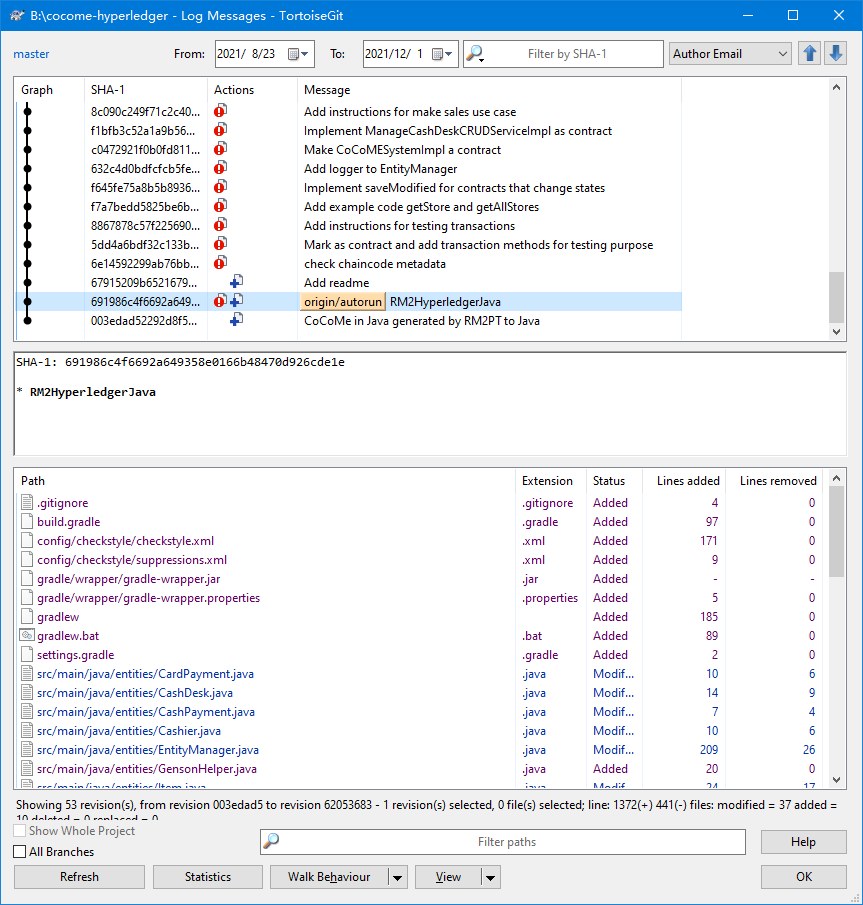
\includegraphics[width=0.9\linewidth]{cocome-hyperledger-log}
\caption{The base of cocome-hyperledger is the JavaFX source code generated by RM2PT. Then RM2HyperLedger automatically converts it to HyperLedger chaincode.}
\label{fig:cocome-hyperledger-log}
\end{figure}

\autoref{fig:cocome-hyperledger-log} shows RM2HyperLedger is able to automatically convert some source code into HyperLedger format, but I have to do more conversions because not all conversion rules have been implemented in RM2HyperLedger. Currently I am collecting my manual conversion rules into RM2HyperLedger, so eventually no manual editing is needed.

Besides the functional implementation, I also worked on requirements validation and test code generation. \autoref{testManageItem} is an example unit test that follows the manage item UML activity diagram. This code ensures all function calls except the last one do not fail, and after each function call, \code{docker stop} stimulates a network node down (because in the actual network any node can leave anytime). Due to the pre- and post-conditions of \code{deleteItem}, this function cannot be called twice, thus reflected in the test code.


\begin{figure}[ht]
\begin{lstlisting}[language=bash, breaklines=true, showstringspaces=false, frame=tb, caption={A Bash function that tests operations in the manage item category}, label=testManageItem]
testManageItem() {
  pci -C mychannel -n cocome --waitForEvent -c '{"function":"ManageItemCRUDServiceImpl:createItem","Args":["1","cookies","10","10","9"]}' || fail

  docker stop "$(docker ps -n 1 --filter 'name=dev' --format '{{.ID}}')"

  peer chaincode query -C mychannel -n cocome -c '{"function":"ManageItemCRUDServiceImpl:queryItem","Args":["1"]}' || fail

  docker stop "$(docker ps -n 1 --filter 'name=dev' --format '{{.ID}}')"

  pci -C mychannel -n cocome --waitForEvent -c '{"function":"ManageItemCRUDServiceImpl:modifyItem","Args":["1","Pepperidge farm cookies","12","5","10"]}' || fail

  docker stop "$(docker ps -n 1 --filter 'name=dev' --format '{{.ID}}')"

  pci -C mychannel -n cocome --waitForEvent -c '{"function":"ManageItemCRUDServiceImpl:deleteItem","Args":["1"]}' || fail

  if pci -C mychannel -n cocome --waitForEvent -c '{"function":"ManageItemCRUDServiceImpl:deleteItem","Args":["1"]}'; then
    fail 'Cannot delete the same item twice'
  fi
}
\end{lstlisting}
\end{figure}

These tests are implemented compatible to GitHub Actions, i.e., GitHub is able to run these tests to verify the correctness of the application. In total, at present three such tests are implemented. \autoref{fig:github-action}~shows one run of these tests on GitHub.

\begin{figure}[ht]
\centering
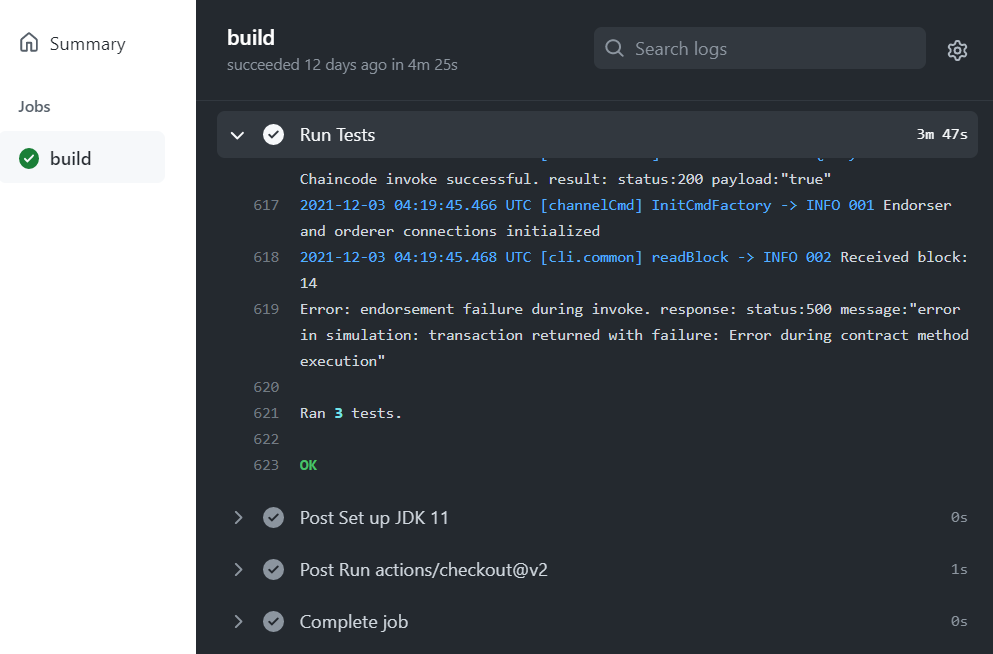
\includegraphics[width=0.9\linewidth]{github-action}
\caption{The code of requirements validation is able to run on GitHub. 3 tests pass.}
\label{fig:github-action}
\end{figure}

	\onehalfspacing\chapter{Publications and Technical Report Produced}
\label{sec:produced-publications}

Q.~Gu and W.~Ke, ``A neural architecture for detecting identifier renaming from
diff,'' in {\em International Conference on Intelligent Data Engineering and
Automated Learning}, pp.~33--44, Springer, 2021.
	\onehalfspacing\chapter{Technology Details}

The technology details on the identifier renaming project has been published in paper ``A Neural Architecture for Detecting Identifier Renaming from Diff'' seen in \autoref{sec:produced-publications}.
This chapter hence presents technology details for the RM2HyperLedger project. I first explain the technology of RM2PT, then transition to RM2HyperLedger.

\section{RM2PT}

The RM2PT program written by Yang is an Eclipse plugin, written in Xtend, a Java dialect. The main input to RM2PT is a \code{.remodel} file, which is a requirement document written in Yang's  domain specific language. \autoref{yang-dls} is an abridged \code{.remodel} file. The exact language specification is unknown, but the contract definition part is in Object Constraint Language (OCL).

\begin{figure}[ht]
\begin{lstlisting}[language={}, breaklines=true, showstringspaces=false, frame=tb, caption={an abridged \code{.remodel} file. The contract definition part is written in OCL.}, label=yang-dls]
UseCaseModel CoCoME {
	UC::processSale() definedBySSD(ProcessSaleSSD) relatedService(ProcessSaleService)
	UC::openCashDesk()

	Actor Cashier {
		processSale
		openCashDesk
		closeCashDesk
	}

	Contract  ManageSupplierCRUDService::deleteSupplier(id : Integer) : Boolean {

		/* definition: find specific Supplier instance by id */
		definition:
			supplier:Supplier = Supplier.allInstance()->any(sup:Supplier | sup.Id = id)

		/* precondition: the instance supplier was found in the system */
		precondition:
			supplier.oclIsUndefined() = false and
			Supplier.allInstance()->includes(supplier)

		/* postcondition: the instance supplier was deleted from the system */
		postcondition:
			Supplier.allInstance()->excludes(supplier) and
			result = true
	}
}

DomainModel CoCoME {
	@AutoCRUD
	Entity ProductCatalog {
		Id : Integer
		Name : String

		[Refer]
		ContainedItems : Item* Association
		[INV]
		inv UniqueProductCatalogId : ProductCatalog.allInstance()->isUnique(p:ProductCatalog | p.Id)
	}
}
\end{lstlisting}
\end{figure}

\begin{figure}[ht]
\centering
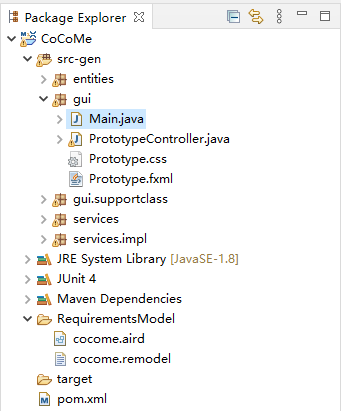
\includegraphics[width=0.5\linewidth]{rm2pt-folder-structure}
\caption{The project structure of a RM2PT project where all Java source code is auto-generated, grouped in the \code{src-gen} folder.}
\label{fig:rm2pt-folder-structure}
\end{figure}

\begin{figure}
\centering
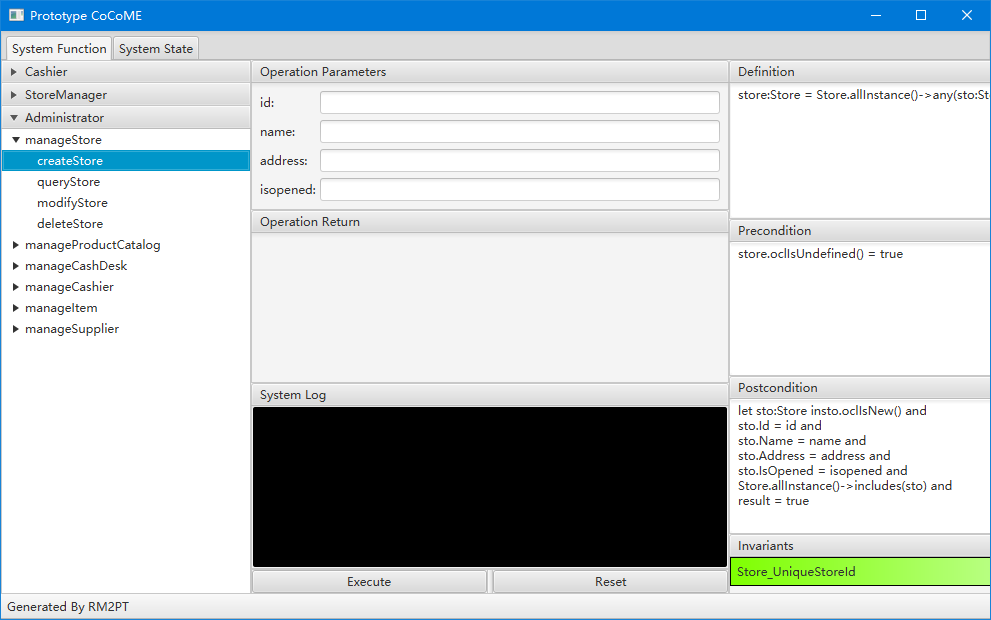
\includegraphics[width=0.7\linewidth]{cocome-javafx}
\caption{Screenshot of the desktop application generated by RM2PT}
\label{fig:cocome-javafx}
\end{figure}


RM2PT thus translates a \code{.remodel} file to a JavaFX project. The project structure is shown in~\autoref{fig:rm2pt-folder-structure} and all Java source code is auto-generated, grouped in the \code{src-gen} folder.
The project is a desktop application with a GUI implemented in JavaFX. \autoref{fig:cocome-javafx}~is a screenshot of the JavaFX prototype.


\section{RM2HyperLedger}

I am currently developing RM2HyperLedger, a program that translates requirements to HyperLedger chaincode.

Unlike RM2PT, RM2HyperLedger is a standalone application written in Java, not relying on Eclipse as many developers use IntelliJ Idea or other IDEs. For now RM2HyperLedger takes as input the \code{.remodel} file and the generated JavaFX code. RM2HyperLedger uses Antlr to analyze Java source code and translate to the HyperLedger Fabric format.

I have encoded the following translation rules in RM2HyperLedger.

\begin{itemize}
\item Add or locate system level identifier (PK) of each entity.
\item Add serialization support to each entity.
\item Store serialized objects to blockchain, and retrieve them by their PK.
\item Rewrite method signatures to fit HyperLedger Fabric format.
\item When a new object is created or an object is deleted from memory, synchronize with the blockchain.
%\item etc.
\end{itemize}

I am still going to formalize and encode more rules, for example
1) when an object is modified, synchronize with the blockchain;
2) rewrite class definition to fit HyperLedger Fabric format;
3) automatically generate test code;
and so on.

\end{appendices}

\end{document}